% !TEX root = main.tex

\section{Ranking the output of Static Analysis}\label{sec:ranking}
% Describing How You Solved the Problem or Answered the Question

% This part of the thesis is much more free-form. It may have one or several sections and subsections. But it all has only one purpose: to convince the examiners that you answered the question or solved the problem that you set for yourself in Section 4. So show what you did that is relevant to answering the question or solving the problem: if there were blind alleys and dead ends, do not include these, unless specifically relevant to the demonstration that you answered the thesis question. 


\subsection{Feedback Rank and Z-Score}

\henrique{This section is named Feedback Rank and Z-Score, and the next Section is named Z-Score. If there is Z-score is not described in this section (but detailed in the next one) it should not be on the title.}
% \textbf{TODO: maybe try a different correlation (author/alert type/?)}
% check vs naive bayes - trade off with speed

Feedback Rank~\cite{correlation_exploitation} combined with Z-Score~\cite{z-ranking} is a simple technique that ranks alerts on the probability of them being actionable.
 It consists of three basic features: package, file, function of the alert being analyzed (though may be extended as needed). 
\henrique{It is very difficult to understand what you mean in the last sentence. Only after reading the next sentence and looking at the Figure below that I got what you meant. You may want to re-write the paragraph as it is confusing}
By constructing a Bayesian Network based on these three features and the history of the project (which alerts have been proven valuable) it produces a probability ranking about which alerts are most useful. \henrique{You should detail the 'history of the project' which is probably one of the key elements to your ranking.}


As explained on the literature review (\cref{lit:fbrank}), Feedback Rank is based on the assumption that bugs and false positives are clustered by code locality. The alerts are divided into two major regions, one that contains mostly true positive, and one that contains mostly false positives. A Bayesian Network (BN) is used to calculate the probabilities of an alert or cluster of alerts belonging to a certain region.

\henrique{You should reference the Figures in your text. Where the Figure bellow fits mostly in the text?}

\begin{figure}[H]
	\centering
	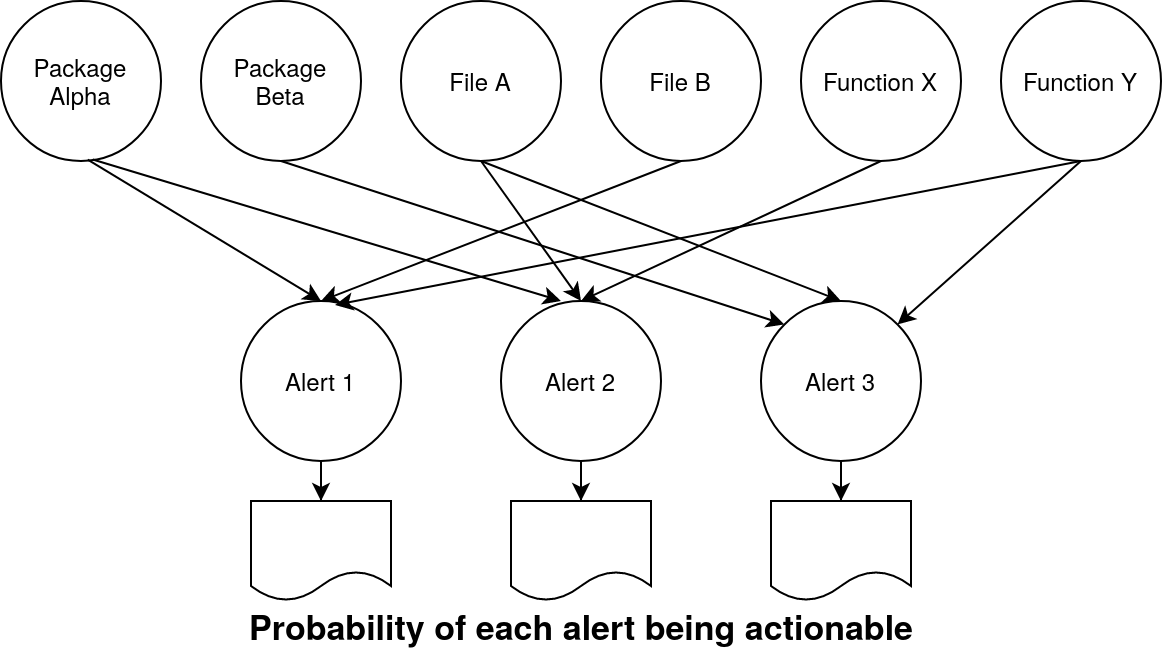
\includegraphics[scale=0.2]{./src/bayes_example.png}
	\caption{Example of a simple Bayes Network for predicting 3 alerts}
\end{figure}

The initial configuration of the network can learned from historical data (extracted as explained on \cref{data_collection}). According to the original authors Feedback Rank is supposed to be an online ranking system: if we inspect a report and know its value, the probabilities of the parents are re-calculated. In this implementation, a static version is used. \henrique{When you write 'According to the original authors' you should provide a reference here. And you say you are going to use a static version but do not describe how that would work.}

To construct the BN, the Pomegranate library was used \cite{pomegranate}, trained with the extracted alert data from the version history. \henrique{Carefull on the overuse of passive voice. The same sentence could be rewritten without it. For example... We use the Pomegranate library~\cite{pomegranate} to construct the BN. Moreover, we trained the BN with extracted alert data from the version history.}


\subsubsection{Z-Score}

\henrique{Carefull on the overuse of passive voice. Every time you write "X is used" try to see if you can rewrite the sentence in active voice as "we use X".}
To break ties when the probabilities provided by the BN are equal between alerts, the Z-Score metric is used based on the number of alerts on the same file. Z-Score is used in Z-Ranking \cite{z-ranking}, which makes use of the observation that the most reliable error reports are those that generated few failed checks and many successful checks, since the actual amount of bugs in code is relatively small (see \cref{lit:zranking} for more details). 

The \textit{z-test} statistic, which measures how far an observed value is from the real population, in this case produces a large positive \textit{z-score} when there are few errors and many successes, and a large negative \textit{z-score} when there are few successes and many errors.

To make use of the Z-Score, an approximation is made. The granularity used for calculating the scores of alerts is based on file level (how many actionable/unactionable alerts of a certain type in a file), instead of the original granularity of the alert (for example an alert that only works on \textit{for loops}). This approximation is made because we do not know for each alert in which code construct it works on. Also, since it is only used as a tie-breaker, a high precision is not indispensable.

\subsection{Detecting Actionable Alerts via Machine Learning}
% classifiers used, how to train (grid search), overfitting, ways to measure

Different techniques focused on automatically classifying alerts in true/false positives or actionable/unactionable alerts, by constructing classifiers based on code or change metrics~\cite{actionable_sa, model_building_actionable}.

Instead of classifying alerts as true or false positives, we focus on Actionable Alerts which are alerts that are deemed important by the developers (not restricted to the type of alerts, but also to the context on which it manifests itself). Actionable alert is a less restrictive definition and makes it easier to collect data. Classifying alerts as true or false would require an oracle or a large and representative dataset generated manually. Moreover, from a developer's perspective, AAs can be more useful. A true positive alert may not be necessarily important to developers and thus be equally useless as a false one (e.g, low severity, no impact on the user side).

We followed the example of Heckman and Williams~\cite{model_building_actionable} to conduct our research since it contains an agglomeration of alert characteristics (AC) collected from other papers.

The workflow, as explained in \cref{data_collection}, consists of iterating through the version history, collecting alerts characteristics and keeping track which alerts disappear (considered as actionable). ACs are then later used as features in ML algorithms with actionability being the target to predict.

We use the scikit-learn library~\cite{scikit-learn} to perform ML experiments in our evaluation.

\subsubsection{Alert Characteristics}

\henrique{Is it supposed to be: "Table X shows the collected features ..." ?}
The collected features can be classified in four main categories: alert information, source code metrics, churn metrics and version history information.

%
%\paragraph{Alert information:} (a) package name (or folder), (b) file name, (c) file extension, (d) alert type, (e) alert category (security, core guidelines...), (f) method signature.
%
%\paragraph{Source code metrics:} (a) number of statements, (b) number of methods, (c) number of classes, (d) cyclomatic complexity.
%
%\paragraph{Version history:} (a) alert open revision, (b) developers who made changes from the open revision of an alert to revision under analysis, (c) file creation revision, (d) file deletion revision, (e) latest modification revision.
%
%\paragraph{Churn metrics:} (a) added lines, (b) deleted lines, (c) growth (added-deleted), (d) total modified (added+deleted), (e) percent modified.
%
%\paragraph{Aggregate characteristics:} (a) total alerts for revision, (b) total open alerts for revision, (c) alert lifetime, (d) file age, (e) alerts for artifact (method, file, package), (f) staleness (amount of time since last change of file, method, package).

\henrique{Where is this table number and title/caption. It is also important that the table is explicitly mentioned on the text.}
\begin{table}[H]
	\centering
	\begin{tabular}{@{}ll@{}}
		\toprule
		\textbf{Feature}            & \textbf{Description}                                               \\ \midrule
		\textit{category}           & Alert category                                                     \\
		\textit{type}               & Alert type                                                         \\
		\textit{function}           & Name of function where alert is located                            \\
		\textit{class}              & Name of class where alert is located                               \\
		\textit{file}               & Name of file where alert is located                                \\
		\textit{package}            & Name of folder where alert is located                              \\
		\textit{openRevision}       & Revision number when alert appeared (default base revision)        \\
		\textit{alertLifetime}      & current revision number - open revision number for alert           \\
		\textit{}                   &                                                                    \\
		\textit{functionSize}       & Number of statements in function where alert is located            \\
		\textit{fileSize}           & Number of statements in file where alert is located                \\
		\textit{nrFunctions}        & Number of functions in file                                        \\
		\textit{nrClasses}          & Number of classes in file                                          \\
		\textit{nrParameters}       & Number of parameters in function where alert is located            \\
		\textit{functionComplexity} & Cyclomatic completicy of function where alert is located           \\
		\textit{}                   &                                                                    \\
		\textit{addedFile}          & number of lines added to file in this revision                     \\
		\textit{deletedFile}        & number of lines deleted from file in this revision                 \\
		\textit{modifiedFile}       & addedFile + deletedFile                                            \\
		\textit{growthFile}         & addedFile - deletedFile                                            \\
		\textit{addedTotal}         & number of lines added in this revision                             \\
		\textit{deletedTotal}       & number of lines deleted in this revision                           \\
		\textit{modifiedTotal}      & addedTotal + deletedTotal                                          \\
		\textit{growthTotal}        & addedTotal - deletedTotal                                          \\
		\textit{}                   &                                                                    \\
		\textit{firstChangeFile}    & Revision number of first file change (default base revision)       \\
		\textit{lastChangeFile}     & Revision number of last file change (default base revision)        \\
		\textit{firstChangePackage} & Revision number of first change in package (default base revision) \\
		\textit{lastChangePackage}  & Revision number of last change in package (default base revision)  \\
		\textit{fileAge}            & lastChangeFile - firstChangeFile                                   \\
		\textit{fileStaleness}      & current revision - last change revision for file                   \\
		\textit{packageStaleness}   & current revision - last change revision for package                \\
		\textit{lastKnownDev}       & Last developer to change file                                      \\
		\textit{mostPresentDev}     & Developer that made most changes to file                           \\ \bottomrule
	\end{tabular}
\end{table}


%\subsubsection{Pre-processing data}
%
%***mostly categorical data -> tree based algorithms\\
%\textbf{***do not use label encoding with nominal data (false order)}\\
%\textbf{***try other encoding techniques}
%
%\paragraph{Label encoding} Some algorithms need data in numerical form. Since most of the features are categorical data, we need a way to convert them to numerical. A simple approach was chosen, label encoding, which assigns an integer to each value of a category. Other approaches such as One-Hot encoding would increase the amount of data a lot (ex. consider one-hot encoding the file where an alert a method is from, which is a feature with high cardinality).
%
%\paragraph{Imbalanced dataset} A quick look at the number of closed or not closed alerts shows that the dataset is heavily unbalanced. In order to train the ML algorithms we need first to balance the dataset. Two main techniques were tried: random undersampling and SMOTE (by using the library from \cite{imblearn}).\\
%
%\textbf{TO DO:}\\
%-cite paper where oversampling works better\\
%-list other metrics\\
%-explain balancing techniques?
%
%\paragraph{Scaling} While for tree based algorithms scaling is not needed, for other algorithms like Logistic Regression, scaling the inputs can make a difference.
%
%\paragraph{Missing values} In some ACs data may be missing, for example...
%
%\paragraph{Feature selection} The features needed to train the models vary from project to project. Since collecting features that have little to no impact on algorithm performance is a waste of resources, techniques can be applied to select the most representative subset of features. Two main techniques were used: PCA and Recursive Feature Elimination.
%\textbf{TODO: COMPARISON FULL FEATURES VS REDUCED}
% correlations?

\subsection{Bug related lines}

Another automatic way to determine which alerts are useful is to check if they pointed to lines that were changed during bug fixes. By doing so, we are regarding as extra valuable those alerts that potentially signaled future bugs. The concept of bug related lines (BRL) is used by Kim and Ernst~\cite{which_warnings}, and by Liang et al.~\cite{automatic_training_set}.

BRLs are calculated as follows:
\begin{itemize}
    \item We start at a base version of the source code and iterate backwards to a target revision. 
    \item If revision under analysis is a bug-fixing revision (contains a bug ID) collect changed/deleted code lines from the version history.
    \item If those collected lines were present in the code at least since the target revision, we consider them bug related lines.
    \item Continue iterating backwards, collecting BRLs. If previous lines that were considered BRL were changed before reaching the target revision, we remove them from the set. 
\end{itemize}

\henrique{Every Figure, table, algorithm, chart, and diagram should be explicitly mentioned in the text. For example, you could put the following sentence below to mention the figure. Figure~\ref{fig:calculating-brls} shows a summarization of the general process we follow to calculate BRLs.}

\begin{figure}[H]
    \centering
    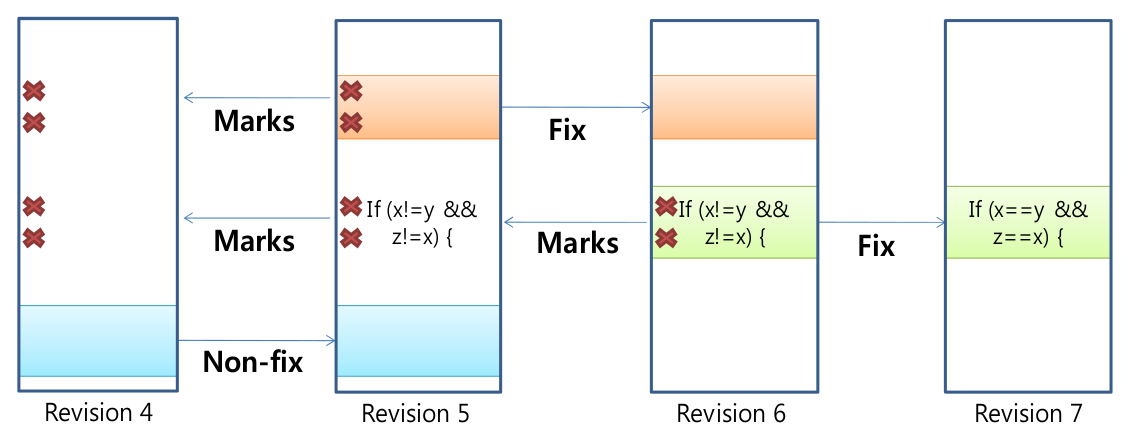
\includegraphics[scale=0.3]{./src/brl_example.png}
    \caption{Calculating BRLs (\cite{which_warnings})}
    \label{fig:calculating-brls} %% *** Put labels in the figures, tables, etc, to make it easier to reference them.
\end{figure}

% generic BRL vs project specific BRL

Since the number of collected lines and warnings can be rather limited, we extend the definition to \textit{Bug Related Methods} (BRM). Namely, we trace in which methods the BRLs belong to and also consider alerts inside those methods as valuable. That allows us to extend the dataset, but also potentially weakens the data by introducing more noise.

Given that the number of alerts collected this way, is a lot less than the total number of alerts, this method is more suited for ranking alert types rather than individual alerts (as used in \cite{which_warnings}).
\henrique{I did not understand what is the relation that makes it better suited for ranking alert types.}

\begin{figure}[ht]
	\centering
	\begin{minipage}{.5\linewidth}
		\begin{algorithm}[H]
			\SetAlgoLined
			\KwData{Collected bug-related alerts and actionable alerts}
			\KwResult{Weighted alert types}
			$\alpha, \beta = x, y$\;
			$w_t = 0 \ for \ t \ in \ alertTypes$\;
			\For{alert in collectedAlerts}{
				$w_t = typeOf(alert)$\;
				\If{alert pointed to a BRL or BRM}{
					$w_t = w_t + \alpha$
				}
				\ElseIf{alert is actionable}{
					$w_t = w_t + \beta$
				}
			}
			$w_t = \frac{w_t}{|alerts \, of \, type \, t|}$
			\caption{Alert type priotitization algorithm}
		\end{algorithm}
	\end{minipage}
\end{figure}

\subsection{Method Bug prediction}

Following the example of Boogerd and Moonen~\cite{static_profiling}, which aims to prioritize alerts based on the execution likelihood of the code pointed by the alert, we present a similar approach. Alerts pointing at potential bugs are the ones that can be considered the most important. The cost of detecting and fixing a bug is much lower if detected early in the development cycle. If we can predict which components will be likely to cause failures in the future, we can prioritize alerts that point to those components.

The appropriate granularity to use for bug prediction is at method level. File level granularity is too broad since a lot of files contain many lines of code, which would result in prioritizing a lot of alerts. On the other hand, finer granularity than method level would be too hard to predict.

We follow the example of Giger et al.~\cite{prediction_method} method. By using a combination of source code and change metrics and by exploiting the version history of the codebase, classifiers can be built that predict bug prone methods.

\begin{table}[]
	\centering
	\begin{tabular}{@{}ll@{}}
		\textbf{Metric Name}          & \textbf{Description}                                                                                                                   \\ \midrule
		\textit{methodHistories}      & Number of times a method was changed                                                                                                   \\ \midrule
		\textit{authors}              & Number of distinct authors that changed a method                                                                                       \\ \midrule
		\textit{stmtAdded}            & Sum of all source code statements added to a method                                                                                    \\ \midrule
		\textit{maxStmtAdded}         & \begin{tabular}[c]{@{}l@{}}Maximum number of source code statements added \\ \\ to a method body for all method histories\end{tabular} \\ \midrule
		\textit{avgStmtAdded}         & \begin{tabular}[c]{@{}l@{}}Average number of source code statements added\\ to a method body per method history\end{tabular}           \\ \midrule
		\textit{stmtDeleted}          & \begin{tabular}[c]{@{}l@{}}Sum of all source code statements deleted from\\ a method body over all method histories\end{tabular}       \\ \midrule
		\textit{maxStmtDeleted}       & \begin{tabular}[c]{@{}l@{}}Maximum number of source code statements\\ deleted from a method body for all method histories\end{tabular} \\ \midrule
		\textit{avgStmtDeleted}       & \begin{tabular}[c]{@{}l@{}}Average number of source code statements\\ deleted from a method body per method history\end{tabular}       \\ \midrule
		\textit{churn}                & \begin{tabular}[c]{@{}l@{}}Sum of stmtAdded - stmtDeleted over all\\ method histories\end{tabular}                                     \\ \midrule
		\textit{maxChurn}             & Maximum churn for all method histories                                                                                                 \\ \midrule
		\textit{avgChurn}             & Average churn per method history                                                                                                       \\ \midrule
		\textit{decl}                 & \begin{tabular}[c]{@{}l@{}}Number of method declaration changes over all\\ method histories\end{tabular}                               \\ \midrule
		\textit{cond}                 & \begin{tabular}[c]{@{}l@{}}Number of condition expression changes in a\\ method body over all revisions\end{tabular}                   \\ \midrule
		\textit{elseAdded}            & \begin{tabular}[c]{@{}l@{}}Number of added else-parts in a method body\\ over all revisions\end{tabular}                               \\ \midrule
		\textit{elseDeleted}          & \begin{tabular}[c]{@{}l@{}}Number of deleted else-parts from a method\\ body over all revisions\end{tabular}                           \\ \midrule
		\textit{cyclomaticComplexity} & Current cyclomatic complexity of method                                                                                                \\ \midrule
		\textit{nestingDepth}         & Current nesting depth of method                                                                                                        \\ \midrule
		\textit{totalStatements}      & Current number of statements in method                                                                                                 \\ \midrule
		\textit{nrPaths}              & Current number of paths in method                                                                                                      \\ \midrule
		\textit{nrDeclarations}       & Current number of declarations in method                            \\\midrule 
	\end{tabular}
\end{table}

% rank alerts in problematic zones higher - combine with BRL?

%\subsection{Combining the techniques}
%% \subsection{Individual alert tuning}
%% zranking cppcore guidelines
%% COMBINE DIFFERENT TECHNIQUES FOR DIFFERENT ALERTS
%
%\subsubsection{How to combine the strengths?}
%% deep learning? make it flexible, learn with time\\
%apply each technique to a subset of the warnings (which is more appropriate)
%
%\subsubsection{Better results?}
%Does it provide better results?


